\documentclass{article}

\usepackage{caption}
\usepackage{graphicx}
\usepackage{float}
\usepackage{enumitem}
\usepackage{hyperref}

\begin{document}
	\tableofcontents
	
	\section{Cell cycle}
	
	\begin{figure}[H]
		\centering
		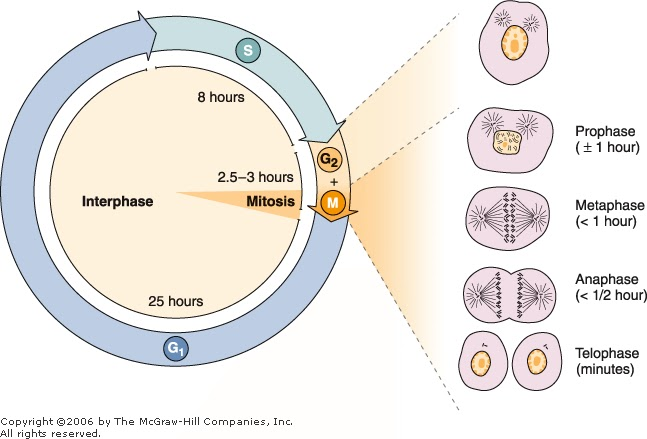
\includegraphics[width=0.8\linewidth]{durations.jpg}
		\caption{\url{https://dehistology.blogspot.com/2011/06/cell-cycle.html}}
	\end{figure}
	
	\subsection{Cdks}
	Cyclin-Dependent Kinases (CDKs) phosphorylate proteins that drive the cell through the cell cycle. This is regulated by
	
	\begin{enumerate}
		\item Synthesis rate of the Cyclins
		\item Ubiquitylation rate of the cyclins (marking them for proteolysis/degradation)
		\item Phosphorylation of the Cdks
		\item CKIs
	\end{enumerate}
	
	\subsection{Cyclins}
	Cyclins activate the CDKs (partially) by forming complexes (see table). There are 4 types of cyclins (A, B, D and E) with various related forms (i. e. D1, D2 and D3 in humans). When characterized by the state of the cell cycle they are active in, they can further be divided into 4 groups: G1/S-Cyclins, S-Cyclins, M-Cyclins and G1-Cyclins.
	
	\begin{table}[h]
		\centering
		\begin{tabular}{|c|c|c|} \hline
			Cyclin & Cdks & Complex \\ \hline
			Cyclin-D & (Cdk4/Cdk6)  & G1-Cdk \\ \hline
			Cyclin-E & Cdk2         & G1/S-Cdk \\ \hline
			Cyclin-A & (Cdk2/Cdk1)  & S-Cdk (MPF) \\ \hline
			Cyclin-B & Cdk1         & M-Cdk (MPF)\\ \hline
		\end{tabular}
		\caption{Cyclines and the Cdks they form complexes with}
	\end{table}

	\begin{enumerate}[label=\textbullet]
		\item G1/S-Cdk initiates the cell cycle in the dormant G1 phase  (yeast: START, mammals: restriction point)
		\item S-Cdk triggers transition from the G1 to the S phase 
		\item M-Cdk triggers transition from the G2 to the M phase 
	\end{enumerate}

	The resulting complex when Cyclin A or B bind to Cdk1/Cdk2 is called the maturation promoting factor (MPF).
	
	\begin{figure}[H]
		\centering
		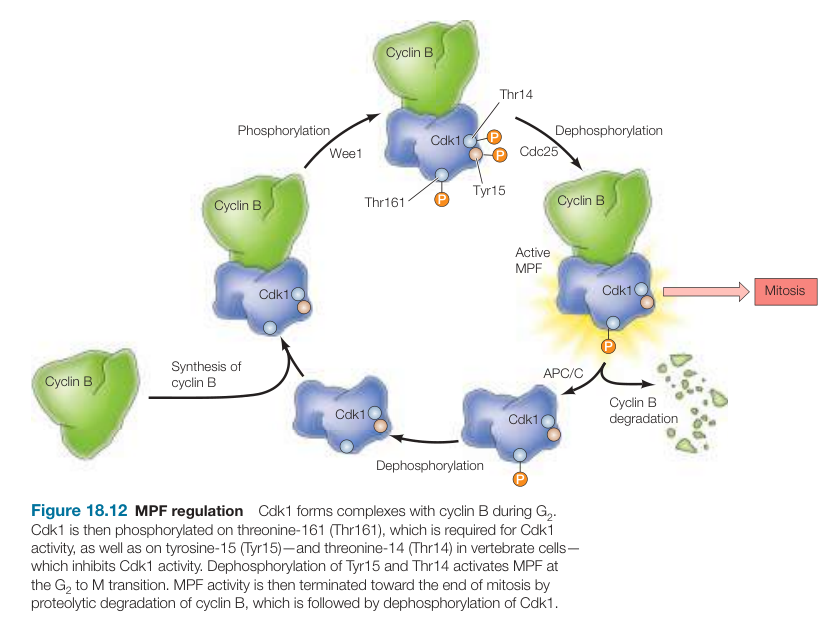
\includegraphics[width=\linewidth]{mpf_regulation_cooper.png}
		\caption{MPF Regulation. The "Phosphorylation" step is carried out by CAK}
	\end{figure}

	Cdk concentration remains mostly constant.\footnote{albert, p. 1093} Concentration of cyclins changes during the cell cycle (see images).
	
	\begin{figure}[H]
		\centering
		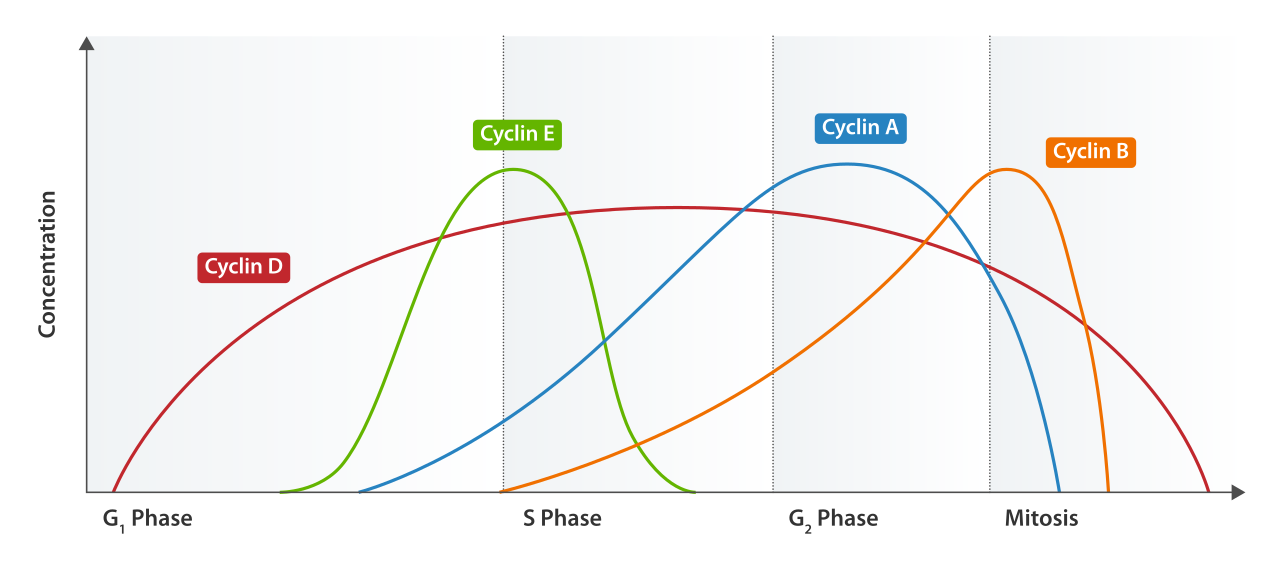
\includegraphics[width=\linewidth]{cyclin_activity_wikipedia.png}
		\caption{Concentration of the cyclins during the cell cycle (wikipedia)}
	\end{figure}
	
	\begin{figure}[H]
		\centering
		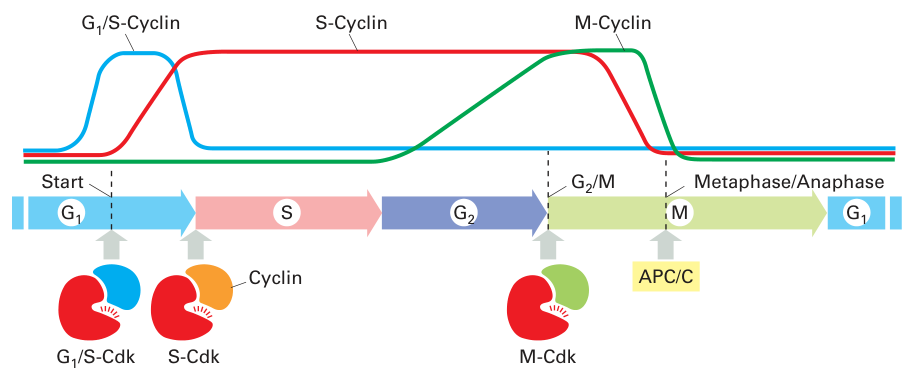
\includegraphics[width=\linewidth]{cyclin_activity_alberts.png}
		\caption{Concentration of the cyclins during the cell cycle (alberts)}
	\end{figure}
	
	\begin{figure}[H]
		\centering
		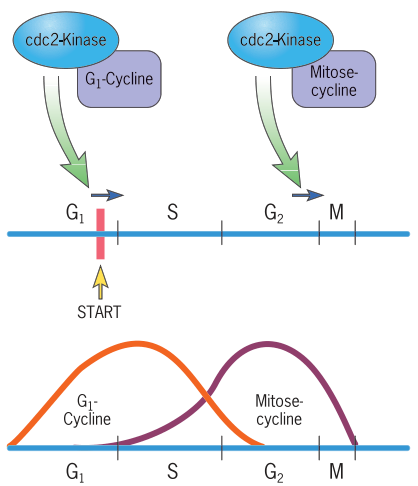
\includegraphics[width=0.8\linewidth]{cyclin_activity_karp.png}
		\caption{Concentration of the cyclins during the cell cycle (karp). cdc2 = cdk1}
	\end{figure}
	
	\subsection{Wee1}
	Wee1 inhibits Cyclin-Cdk complexes by phosphorylation, causing a delay of the M-Phase so that the cell can grow. If Wee1 is defective, the cells transition directly from S- to M-Phase without the growth in the G2 phase, resulting in \textit{wee} little cells :)
	
	\subsection{Cdc25}
	Cdc25 activates the MPF that was previously inactivated by Wee1. It dephosphorylizes Thr14 and Tyr15. Mammals have 3 related forms Cdc25A, B and C.
	
	\subsection{APC/C}
	The anaphase-promoting complex/cyclosome (APC/C) is a ubiquitin ligase and triggers transition from the metaphase to the anaphase by ubiquitylation of securin and Cyclin-A/Cyclin-B, marking them for proteolysis. Once they are destroyed, the MPF is no more.
	
	\subsubsection{Cdc20}
	Binds with APC/C in mitosis to specify target proteins.
	
	\subsubsection{Cdh1}
	Binds with APC/C in late mitosis/G1 to specify target proteins.
	
	\subsection{SCF}
	Skp, Cullin, F-box containing complex is another ubiquitin ligase. SCF ubiquitylates CKIs in the late G1 phase, thus activating S-Cdks; it's also responsible for proteolysis of G1/S-Cdks in the early S phase. Marks p27. Typically requires phosphorylated targets.
	
	\subsubsection{F-Box-Proteins}
	Exchangeable part of the SCF, specifying the target protein. There are more than 70 genes coding for F-Box-Proteins.\footnote{alberts, p. 178}
	
	\subsection{CKIs}
	Cdk inhibitors (CKIs) inhibit Cyclin-Cdk complexes by binding to them (mostly G1/S- and S-Cdks). There are 2 families of CKIs, binding to different Cdks and Cyclin/Cdk complexes:
	
	\begin{figure}[H]
		\centering
		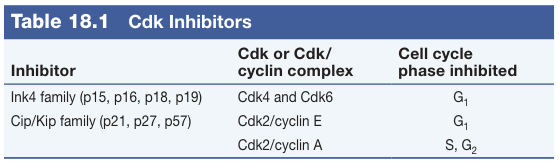
\includegraphics[width=\linewidth]{ckis_cooper.png}
		\caption{CKI families and their targets}
	\end{figure}

	\subsubsection{p27}
	Inhibits Cdks in G1. Gets phosphorylated by Cdk1, causing it to be marked for proteolysis (by SCF or APC/C?). 
	
	\subsubsection{p21}
	Inhibits G1/S-Cdk und S-Cdk if DNA damage occured.
	
	\subsubsection{p16}
	Inhibits G1-Cdk in G1. Frequently inactive in cancer cells.
	
	\subsection{CAK}
	CDK-activating kinase (CAK) activates the cyclin-CDK complex.\footnote{\url{https://en.wikipedia.org/wiki/CDK-activating_kinase}}

\end{document}